\section{Текстээс зураг үүсгэх}
\subsection{Database дээр зурагний мэдээлэл хадгалах table нэмэх}
Database-н table дээр өөрчлөлт оруулахдаа бид sqlalchemy ашиглаж байгаа ба доор бичсэн моделийн дагуу бид migrate хийх юм. Үүний тулд back-end ажиллаж байгаа Docker container-лүү shell нээж төслийн root хэсгээс
\begin{lstlisting}[language=bash]
	alembic revision --autogenerate -m "your commit message"
\end{lstlisting}
гэсэн коммандын ашиглан өөрлөлт оруулах мэдээллиг үүсгэн. Дараа нь
\begin{lstlisting}[language=bash]
	alembic upgrade head
\end{lstlisting}
комманд хийснээр Датабазын модел бүрэн өөрчлөгдөнө.

\begin{lstlisting}[language=Python,caption={Table-рүү оруулсан өөрчлөлт},frame=single]
	class User(Base):
		# ...
		# Other table information

		text_title_string = Column(String(255), nullable=False, default="")
		text_title_color = Column(String(255), nullable=False, default="#000000")
		text_title_font_size = Column(Integer, nullable=False, default=0)
		text_title_font_name = Column(String(255), nullable=False, default="")
		text_title_is_vertical = Column(Integer, nullable=False, default=0)
	\end{lstlisting}

\subsection{API үүсгэх}
Back-end дээр API үүсгэхэд анхаарах хэдэн зүйл бий.
\begin{enumerate}
	\item Validation хийх ингэснээр хэрэглэгчээс ирсэн мэдээллийг шалгаж нэг ёсондоо ажиллахад  ямар нэгэн асуудалгүй болгож байгаа юм. Хэрэв буруу мэдээлэл хүсэлт маягаар ирвэл \textbf{
		      422 Unprocessable Entity}
	      гэсэн хариу буцаана.

	\item Dependency injection байдлаар user-н token-г шалгана ингэснээр хэрэглэгчийн нэвтрэлтийг шалгаж байгаа юм. Хэрэв хэрэглэгч нэвтрээгүй бол \textbf{
		      401 Unauthorized}


\end{enumerate}
Хэрвээ ямар ч асуудалгүй бол шаардлагатай үйлдлүүдийг гүйцэтгэж, хэрэглэгчид хэрэгтэй мэдээллийг буцаана.
\subsubsection{Зураг буцаан илгээх}
Гэвч зургийг буцаан илгээх нь харьцангуй төвөгтэй. Гол учир нь гэвэл зургийг шууд стринг байдлаар явууллаа гэж бодоход том зураг бол өгөгдлийн хэмжээ 33 хувиар ихэснэ үүнээс гадна. Зургийг нэг доор боловсруулж байгаа тул удаан интернеттэй хэрэглэгчийн хувьд зургийг харахгүй хоосон дэлгэц маш удаанаар ширтэх юм.

Харин зургийг хэрэглэгч рүү явуулах хамгийн шилдэг арга бол урсгал маягаар явуулах буюу Stream хэрэглэгчид илгээх юм, ингэснээр ямар нэг илүүдэл хэмжээний файл явуулахгүй, яг тухайн зургийг хэрэглэгчийн интернэтийн хурданд тааруулах бага багаар явуурлах боломж бүрдэх юм, үүний үр дүнд хэрэглэгч зургийг бага багаар уншиж байгааг нь дээрээс нь харах гэх мэт маш олон давуу талтай.
\begin{lstlisting}[language=Python,caption={Зураг буцаан user-лүү илгээх endpoint},frame=single]
	from fastapi import APIRouter, Depends, status
	from sqlalchemy.orm import Session
	from app import schemas
	from app.feature.pillow import pillow_text_generator, preview_text
	from app.models.user import User
	from app.v1 import deps
	router = APIRouter()
	
	@router.post("/", status_code=status.HTTP_201_CREATED)
	def pillow_text(
			*,
			obj_in: schemas.PillowBase,
			db: Session = Depends(deps.get_db),
			_: User = Depends(deps.get_current_user),
	):
			return preview_text(
					text=obj_in.text,
					is_vertical=obj_in.is_vertical,
					color=obj_in.color,
					font_size=obj_in.font_size,
					strokewidth=obj_in.stroke_width,
					bordered=obj_in.bordered,
					PPI=obj_in.PPI,
			)
	\end{lstlisting}

\subsection{Фронтэнд хөгжүүлэлт}
\subsubsection{Дахин ашиглагдах компонент үүсгэх}
Орчин цагийн Фронтэнд хөгжүүлэлтэнд хамгийн түгээмэл ашиглагддаг филсофи бол бүрэлдэхүүн хэсгүүдийг аль болох олон жижиг хэсгүүдэд хувааж дараа нь тэдгээрийг ахин ашиглах явдал юм.

\begin{lstlisting}[language=JavaScript,caption={ProductArea компонент ашигласан байдал},frame=single]
	<div class="relative">
	<ProductArea ref="text_title" v-model="text_title_string" title="商品タイトル" identifier="1"
		:default_text="text_title_string" :default_radio="text_title_is_vertical"
		@textChanged="prod_area_handler" />
	<p v-if="text_title_string_error" class="error-message break-line absolute top110">
		商品タイトルを入力してください
	</p>
</div>
<ProductArea ref="text_copy" v-model="text_copy_string" title="キャッチコピー" identifier="2"
	:default_text="text_copy_string" :default_radio="text_copy_is_vertical"
	@textChanged="prod_area_handler" />
<div class="py-20"></div>

	\end{lstlisting}
	
	\begin{figure}
		\centering
		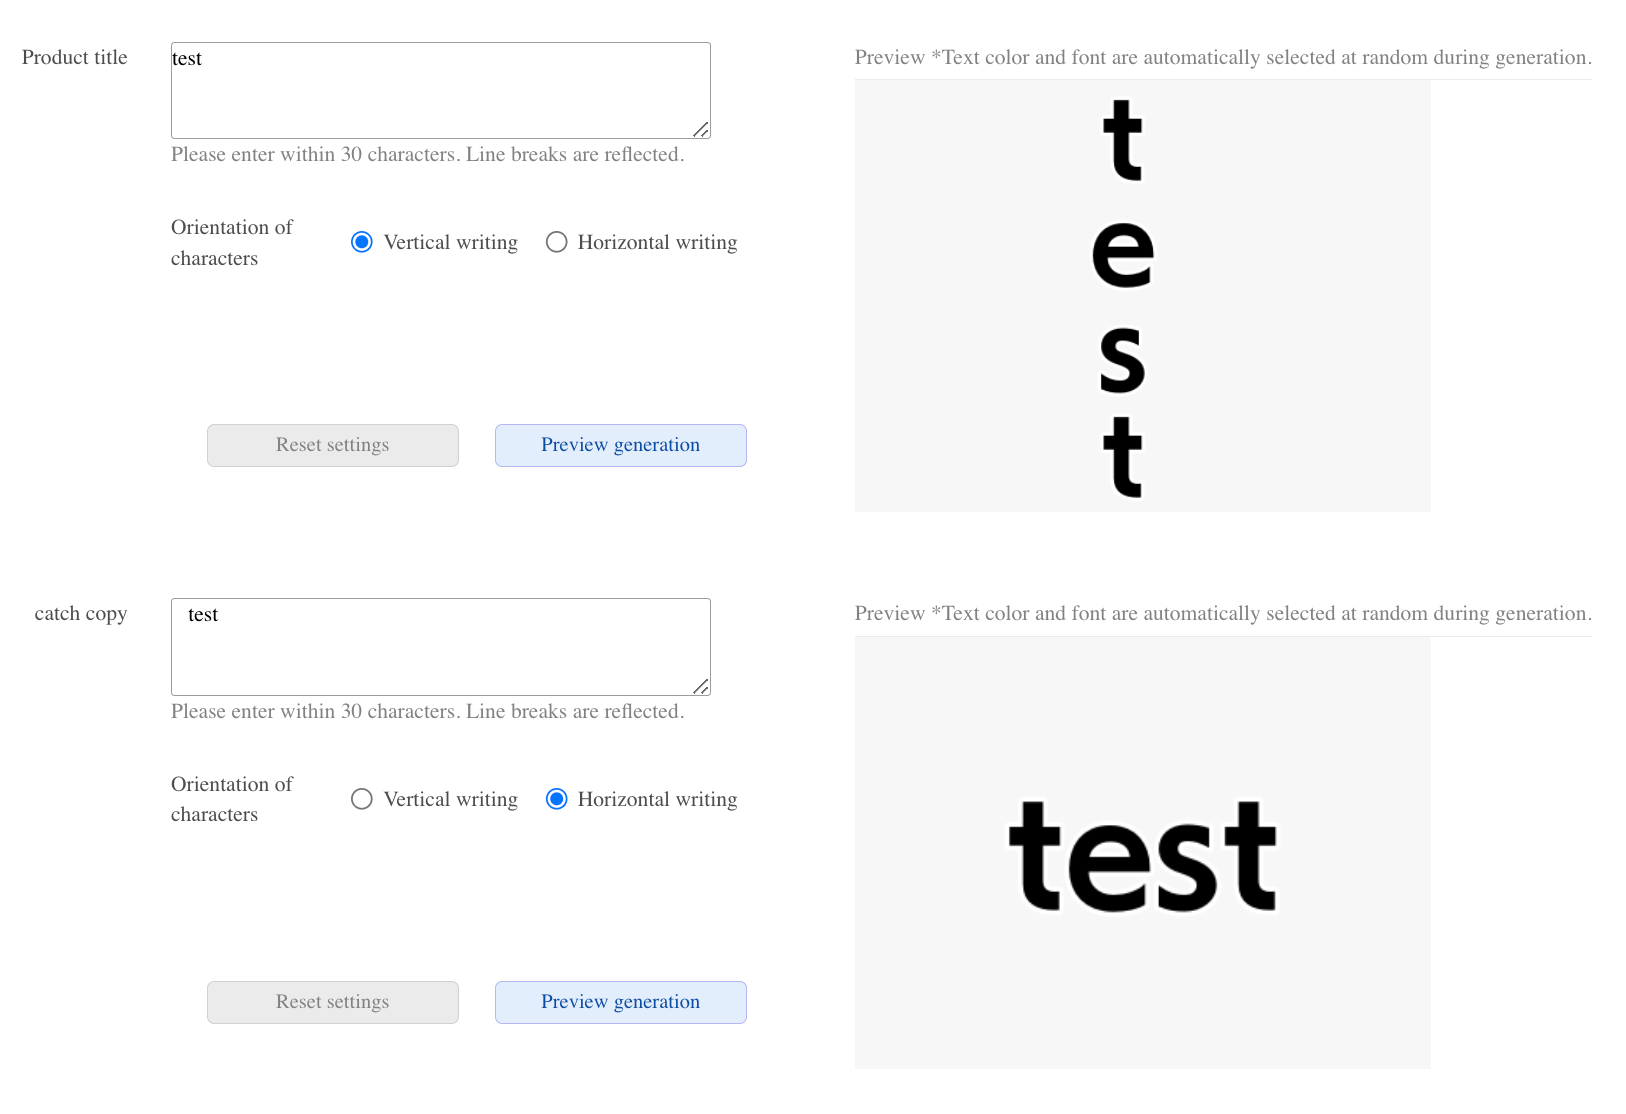
\includegraphics[scale=0.3]{src/pictures/front.png}
		\caption{Алгоритм}
	\end{figure}

\subsection{Үүсгэсэн API дуудах}
Энэхүү endpoint-руу user үүсгэх зурагнийхаа текст мэдээллийг JSON хэлбэрээр POST хүсэлт явуулна. Фронтэнд-с үүсгэсэн Эндпойнт ашиглахдаа responseType-г нь arraybuffer болгож байгаа юм ингэснээр бейс64 (base64) зургийг интернетээр явуулснаас харьцангуй бага нөөц (bandwidth) ашиглах юм. Үүний дараагаар авсан өгөгдлөө задалж (decode) хийж бейс64 зураг болгон хэрэглэгчид харуулна.


\begin{lstlisting}[language=JavaScript,caption={Endpoint дуудах function},frame=single]
	async preview_text_to_image({ _ }, { data }) {
    const result = await this.$axios.post(`text_image/`, data, {
      responseType: 'arraybuffer',
    })
    if (result.status === 200) {
      const b64 = btoa(String.fromCharCode(...new Uint8Array(result.data)))
      const imgData = 'data:' + result.headers['content-type'] + ';base64,' + b64
      return imgData
    } else {
      console.log('error')
    }
  },
\end{lstlisting}

\section{Business logic-г хийх}
Ямар ч request client талаас ирж болох учраас үүнийг сервер дээр боловсруулахын өмнө, validation хийх нь зөв билээ. Үүний тулд Pydantic ашиглаж байгаа юм. Pydantic нь Python дээр зориулсан validation library юм. Үүнийг ашиглан бид үүсгэсэн PillowBase class-н мэдээллийг шалгаж байгаа юм. Хэрэв буруу мэдээлэл ирвэл 422 Unprocessable Entity гэсэн хариуг буцаана.
\begin{lstlisting}[language=Python,caption={Pydantic Validator},frame=single]
	from pydantic import BaseModel
	class PillowBase(BaseModel):
    text: str
    font_path: str
    is_vertical: bool = False
    font_size: Optional[int] = 90
    color: Optional[str] = "#000000"
    bordered: Optional[bool] = True
    stroke_color: Optional[str] = "#ffffff"
    stroke_width: Optional[int] = 3
    gaps: Optional[int] = 3
    PPI: Optional[int] = 300
\end{lstlisting}
Өмнөх API-г зөвхөн хэрэглэгч ямар хэлбэр дүрстэй зураг үүсгэснээ харах зорилготой байсан бол яг production орчинд хэрвээ тэрхүү үүсгэсэн зураг нь таалагдсан бол, текстээс үүсгэсэн зураг материалд ашиглахад тэс өөр логик ашиглах юм.

\subsubsection{Үүсгэсэн зургийг s3-д хадгалах}

\begin{lstlisting}[language=Python,caption={Үүсгэсэн зургийг s3-д хадгалах},frame=single]
	def get_boto3_client():
    global _s3_client

    if not _s3_client:
        if settings.IS_LOCAL:
            _s3_client = boto3.client(
                "s3",
                aws_access_key_id=settings.AWS_ACCESS_KEY_ID,
                aws_secret_access_key=settings.AWS_SECRET_ACCESS_KEY,
            )
        else:
            _s3_client = boto3.client("s3")
    return _s3_client

	def upload_file_object(object_file, file_name: str, bucket: str = settings.GENERATION_S3_BUCKET):
    # Upload the file object
    s3_path = os.path.join(bucket, file_name)
    try:
        s3_client = get_boto3_client()
        s3_client.upload_fileobj(object_file, bucket, file_name)
    except ClientError as e:
        logging.error(e)
        return False, s3_path
    return True, s3_path

\end{lstlisting}



\begin{figure}
	\centering
	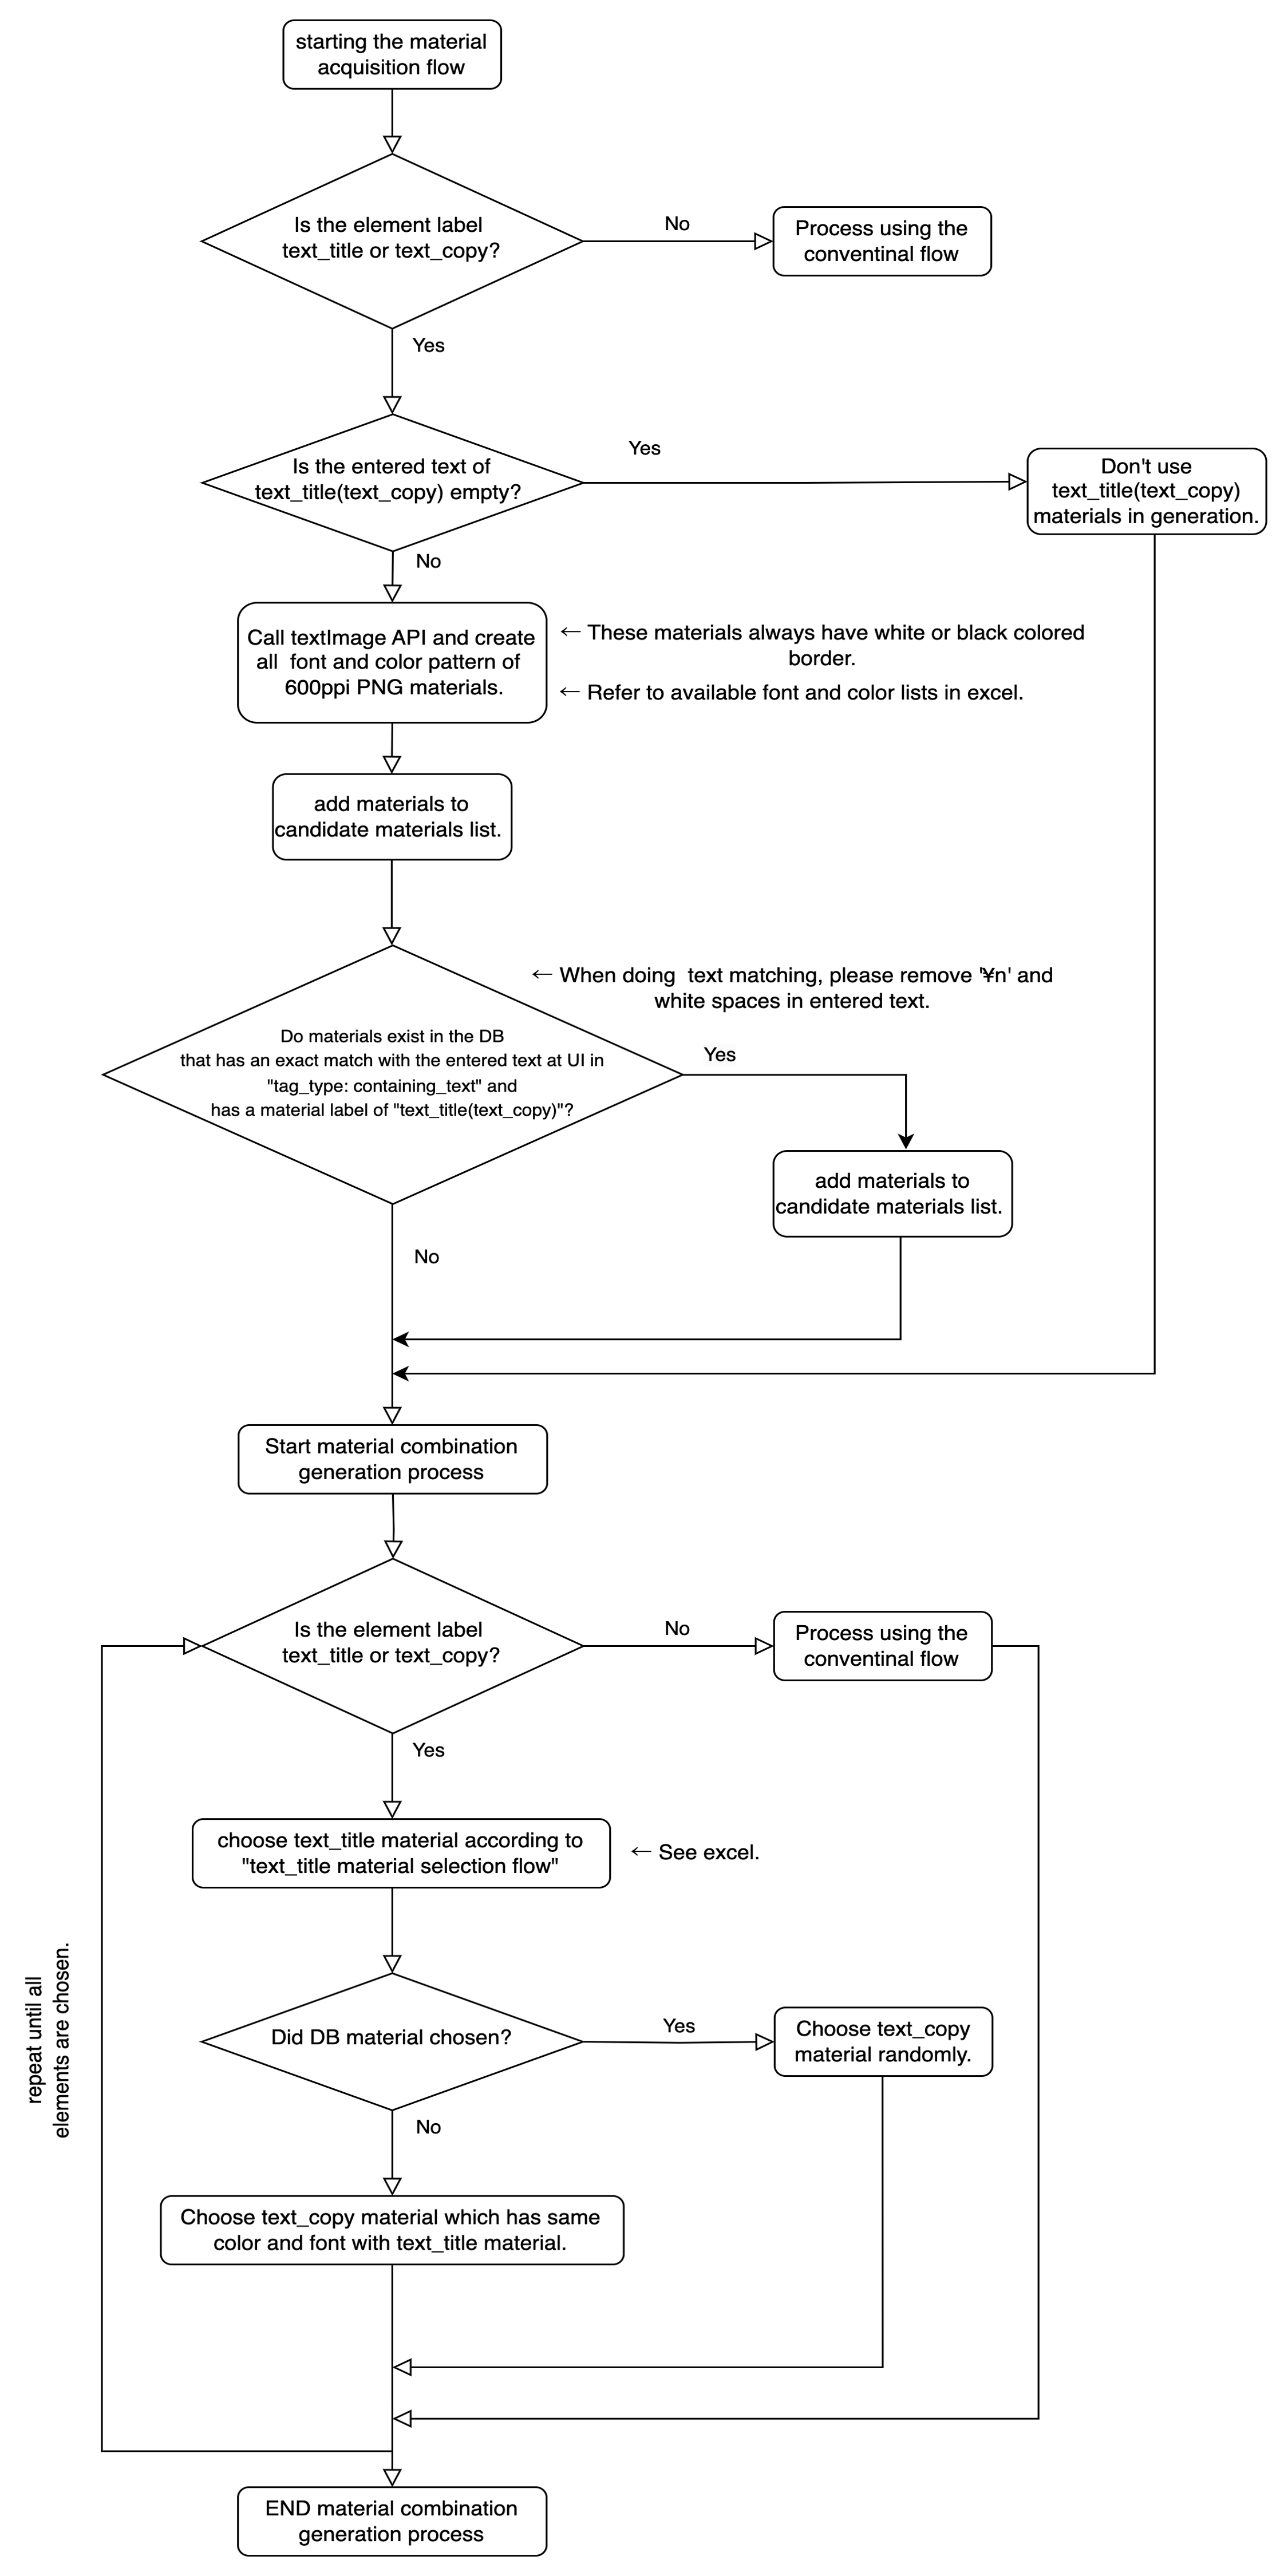
\includegraphics[scale=0.6]{src/pictures/algorithm1.png}
	\caption{Алгоритм}
\end{figure}

\begin{figure}
	\centering
	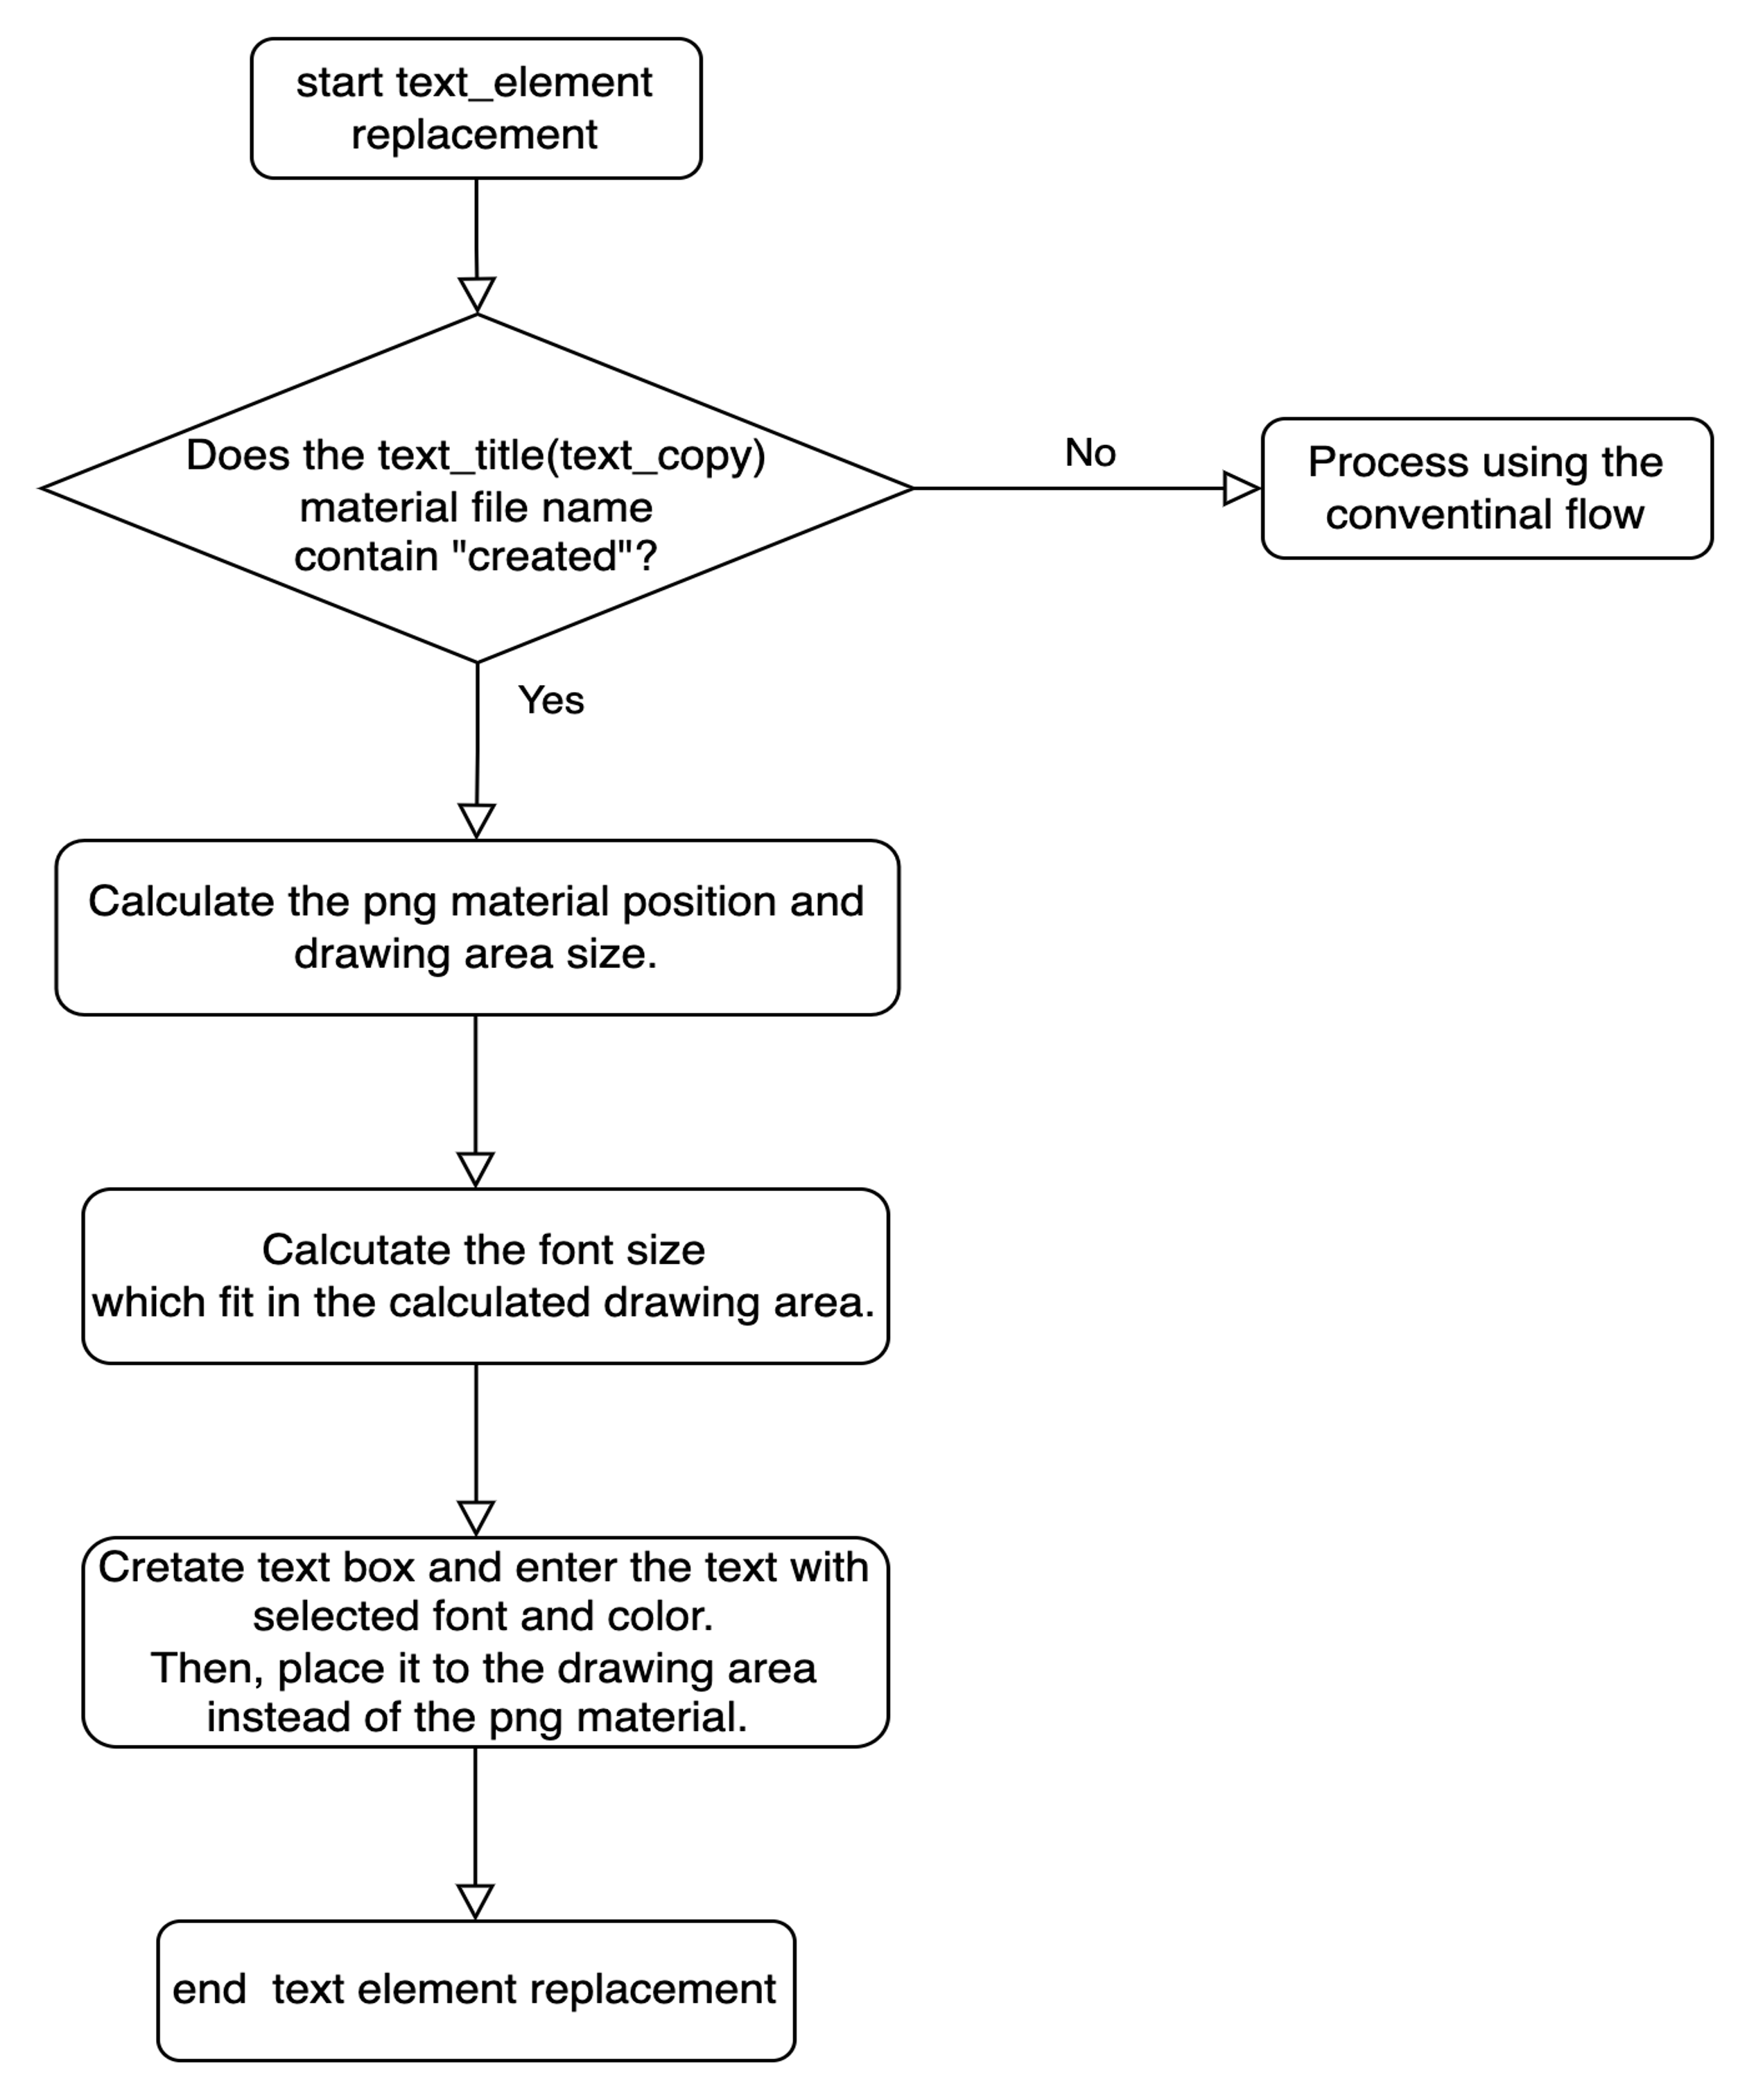
\includegraphics[scale=0.6]{src/pictures/algorithm2.png}
	\caption{Алгоритм-2}
\end{figure}

\begin{figure}
	\centering
	\includegraphics[scale=0.28]{src/pictures/algorithm3.png}
	\caption{Алгоритм-3}
\end{figure}




\subsection{Алгоритмын тайлбар}
Дээрх зурганд харуулсан Алгоритмыг ерөнхийд нь тайлбарлавал, хэрэглэгчийн зураг үүсгэхийг хүссэн тексттэй адилхан агуулгатай өгөгдөл database дээр байгаа эсэхийг шалгах юм. Хэрэв тийм өгөгдөл олдвол тухайн өгөгдлийн цаашид үүсгэх шошгонууд дээрээ жин өгч магадлал тооцон ашиглах юм.
Ингэхдээ текстээс зураг үүсгэдэг алгоритмыг ашиглан 8 өнгө 3 фонт дээр төрөл бүрийн зурагнууд үүсгэж түүнийгээ database дээр олдсон зурагнуудтай нийлүүлэн магадлал тооцно.

\begin{lstlisting}[language=Python,caption={Сонголт хийх код},frame=single]
	if registered_materials_from_db:
	item_list.extend([black, other, db_item])
	item_weight.extend([0.7 * 1 / 3, 0.3 * 1 / 3, 1 / 3])
else:
	item_list.extend([black, other])
	item_weight.extend([0.7, 0.3])
\end{lstlisting}


\subsection{Ажиллах дараалал}
\begin{enumerate}
	\item Хэрэглэгчийн оруулсан текстээс \verb|\n| ялгаж хэдэн мөр байхыг гаргана.
	\item Хэрэглэгчийн оруулсан фонт мөрийн тоо, нэг мөр дэх үсгийн тооноос хамаарч өөр өөр байх хоосон зургуудийг үүсгэнэ.
	\item Хоосон зургуудруугаа текстийг нэг нэгээр нь нэмнэ.
	\end{enumerate}